\epigraph{\textit{"It's good, unless you have vertigo."\\"\dots are you talking about PhD?"}}

\section{Why Photovoltaic}

\paragraph{Abundance} The total solar irradiance hitting the outer Earth atmosphere is around \SI{1361}{\watt\per\square\metre},\cite{Kopp2011} which, considering our planet cross section area, makes \SI{1.6e17}{\watt}.
Nature conveys this energy in plenty of ways, including the generation of every renewable and most of non-renewable energy sources.
Solar energy is effectively the primary energy source for our planet's ecosystem, so it's the most interesting source of energy for human usage.

\paragraph{Availability} Its ubiquitous availability can be the leverage for some degree of economical power levelling across different regions of the planet.
This is even more interesting when considering that most of the regions where life quality is seriously affected by economy (represented in \cref{fig:world_map-HDI} by the Human Development Index) have abundance of solar irradiation (represented in \cref{fig:world_map-PVOUT} by the ratio between the photovoltaic electric energy that can be obtained over the nominal power of an installed solar panel).

\begin{figure}%[!hbtp]%
	\centering
	\begin{subfigure}[b]{1\textwidth}
		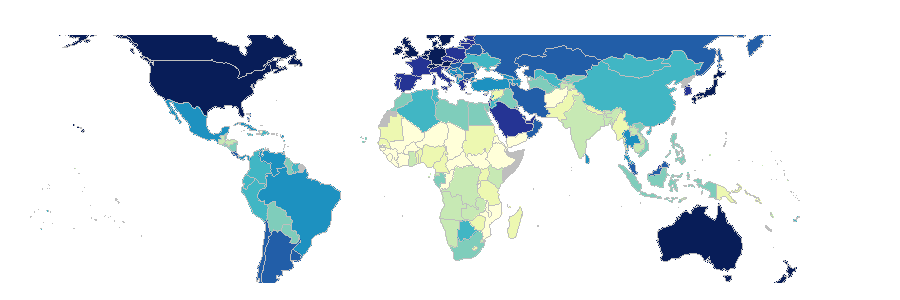
\includegraphics[width=1\textwidth]{world_map-HDI/world_map-HDI.pdf}
		\subcaption{Human development index by region}\label{fig:world_map-HDI}
	\end{subfigure}

	\begin{subfigure}[b]{1\textwidth}
		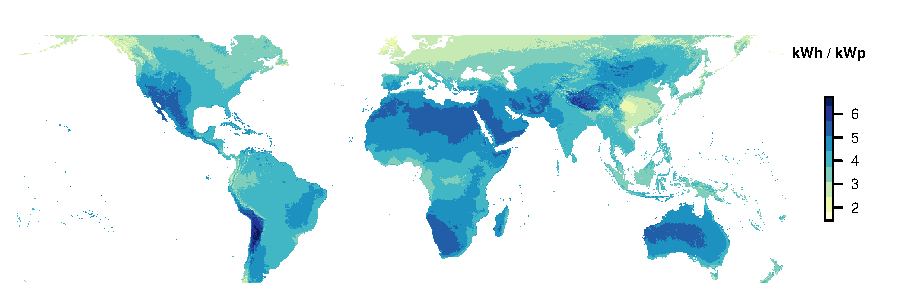
\includegraphics[width=1\textwidth]{world_map-PVOUT/world_map-PVOUT.pdf}
		\subcaption{Daily photovoltaic electricity potential}\label{fig:world_map-PVOUT}
	\end{subfigure}

	\begin{subfigure}[b]{1\textwidth}
		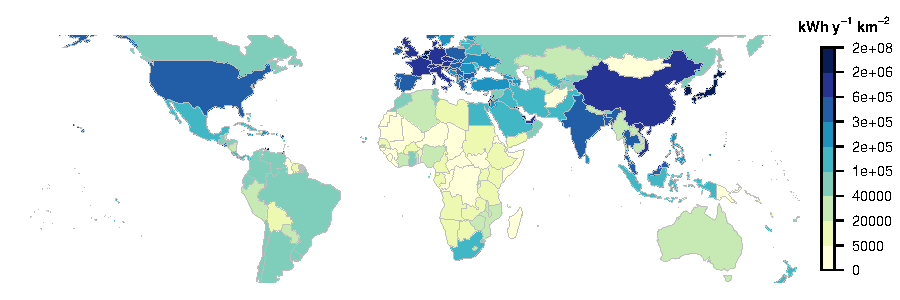
\includegraphics[width=1\textwidth]{world_map-electrical_vs_land/world_map-electrical_vs_land.pdf}
		\subcaption{Yearly electricity consumption over region land area}\label{fig:world_map-electrical_vs_land}
	\end{subfigure}
	\mycaption[Geographical distribution of development, sunlight and consumption.]{Data in (\textbf{a}) represent the human development index:
		"a summary measure of average achievement in key dimensions of human development: a long and healthy life, being knowledgeable and have a decent standard of living"
		from UNDP\cite{UNDP2018} (missing data in grey); data in (\textbf{b}) represents the photovoltaic electricity potential: considering a photovoltaic module installed in a region, is the ratio between the average daily produced energy, in kWh, and the nominal power, or nameplate capacity, of the installed module;\cite{Solargis2018} data in (\textbf{c}) represents the yearly electricity consumption\cite{CIAa} (comparing total electricity generated annually plus imports and minus exports) on a country scale divided by country land surface,\cite{CIA} expressed in kilowatt-hours per year per square kilometre.}\label{fig:world_map}


\end{figure}

\paragraph{Resilience} Photovoltaic is the electric energy production method that best matches a distributed and decentralized network model, with the only single-point-of-failure being the climate variability.
Combined with accumulation (needed for night time usage) and with other energy sources, it can be the pivot of a completely resilient electric energy provisioning system.

\paragraph{More energy is not enough} It is intuitive that increasing the energy production is a high-price solution to the growing energetic demand.
Indeed, in some regions a decrease in the electricity consumption has to be included for a long-term solution.
For example, a study\cite{Margolis2016} reports that if every rooftop (not considering utility-scale solar facilities) in United States of America was covered with solar panel, just the 39~\% of its nowadays national consumption would be covered.
In \cref{fig:world_map-electrical_vs_land} we can see how electricity consumption density is greatly inhomogeneous and comparing with the photovoltaic potential map in \cref{fig:world_map-PVOUT}, it is evident that such a problem is shared with many other poorly insulated but energy eager regions.
Both an increase in machinery's efficiency and a change in life-style can be part of the solution, following the example and thinking at life-style, in USA the per capita energy usage is more than twice the European average, and five times the Latin America average.\cite{IEA}

\paragraph{And more research is needed} Every source of electrical energy we can think of works via the conversion of motive power (a flow of steam, wind, or water, waves, tides...) to electricity, which relays on the well established electric generator. Except photovoltaic energy. This very simple difference already hints for the huge conceptual and technological step required by photovoltaics as compared to other electrical energy sources.

% transducer

\section{PhotoVoltaic Effect}

\paragraph{Light absorption}

\paragraph{Exciton generation}

\paragraph{Exciton splitting}

\paragraph{Charge drift and charge diffusion}

\paragraph{Charge collection}

\paragraph{Electromotive force}

\section{Perovskite Solar Cells}

Perovskite solar cells is a relatively new player in the photovoltaics world, existing just since 2009 CITE OLD GUYS. In relatively short time, see \cref{fig:nrel_chart}, these kind of devices reached a record efficiency of 20.9~\% CITE GREEN2019 with reports of even higher efficiencies (23.7~\% CITE GREEN2019 JIANG2017).


\begin{SCfigure}
	\centering
	\includegraphics[width=0.5\textwidth]{nrel_chart/pv-efficiencies-2019-01-03.pdf}
	\mycaption[NREL chart of "Best Research-Cell Efficiencies"]{Just the Perovskite cells (not stabilized) results have been reported.}\label{fig:nrel_chart}
\end{SCfigure}


\paragraph{Perovskite Absorber Synthesis}

The preparation of this hybrid semiconductor via spin coating and annealing at low temperature is extremely easy and convenient for small-scale research purposes. From my point of view, what most affects the perovskite research is the lack of reproducibility, likely caused by the extremely sensible crystallization during the annealing phase. In literature various reports of completely different results obtained from perfectly identical synthesis can be found\cite{Pockett2015,Gottesman2014}. This issue is being addressed recently with the publication of more reliable and complete fabrication proceduresCITE SALIBA2018.

\paragraph{Ionic migration}

The presence of charged and mobile ionic species have been demonstrated in various kind of hybrid lead halide perovskite materials, via \gls{kpfm}\cite{Birkhold2018} XXXXXXXXXXXXXXXXXX. The presence of mobile ions has been demonstrated also in absence of current-voltage hysteretic behaviour\cite{Calado2016,Jacobs2018}. It has also been demonstrated that for \gls{mapi} the majoritarian mobile species is the iodine vacancy XXXXXXXXXXXXXXXX SENOCRATE2017 and has been excluded a significant contribution from methylammonium ionsCITE SENOCRATE2018 SENOCRATE2017.

\paragraph{Stability}
The stability of the perovskite solar cells is the number one blocker to commercialization. Its keystone has still to be identified. An interesting investigation is being carried on by CITE Ceratti regarding the release of a proton by methylammonium cation when in contact with non-acidic materials, and thus leaving the perovskite crystal structure. This could explain the reports about the beneficial addition of acids in perovskite precursors solution, mainly by Snaith group CITE 10.1016/j.joule.2017.09.009 10.1038/ncomms10030 10.1038/ncomms13303.

\paragraph{Characterization}

The characterization techniques for perovskite solar cells and the relative interpretation evolved from the techniques and theory built around \gls{osc} and \gls{dssc}. This pre-existing framework has been widely used in literature for perovskite solar cells. Unfortunately, perovskite solar cells are different enough from \gls{osc} and \gls{dssc} to doom the utility of most of these observations. In the past few years, the theoretical framework has been expanded and should finally enable the perovskite community to re-interpret and re-design the solar cells characterization techniques. This thesis includes some of the accepted concepts and some novel proposals about the new interpretation of the classical characterization techniques when used on perovskite solar cells.

\section{Efficiency Limiting Factors}

\paragraph{Charge recombination types}

\section{Background and Related Work}\label{sec:background}

\subsection{Perovskite Solar Cells}

\subsection{Hole Transporting Materials}

\subsection{PhotoPhysical Studies and Techniques}

\subsection{Modelling and Relevant Physics}


\section{Aims}